\subsection{Resolution}

The resolution phase has the task to search for every possible construction of an expression which has the given type. 
It considers all values in the given scope as the candidate leaf values for expression synthesis.
Considering such a general scenario leads us directly to the type inhabitation problem \cite{EPFL-REPORT-170040,Urzyczyn:1997:ITL:645893.671612}.
\begin{definition}
\label{def:inhabitation_problem}
Type inhabitation problem:
given a desired type $T$, and a type environment $\Gamma$ (a set of values and their types), find an expression $e$ of the type $T$, i.e. find an expression such that $\Gamma \vdash e : T$.
\end{definition}
More specifically, the goal of the resolution phase is to solve the type inhabitation problem - for a input type $T$, to use theorem proving techniques to search for proofs of construction of all valid expressions $e$ of type $T$.
These proofs are then forwarded to the code generations phase which uses them to produce synthesises syntactically correct code snippets.

InSynth gets the necessary inputs from the IDE and the resolution phase computes $\Gamma$ by looking at all program declarations and visible API from the position of the cursor in the editor, looks up $T$ by examining the declared type appearing left of the cursors in the editor and finally solves the type inhabitation problem.

The structure of the phase done by the proof resolution module is depicted in Figure \ref{fig:InSynth_resolution_steps}.

\begin{figure}[ht]
\centering
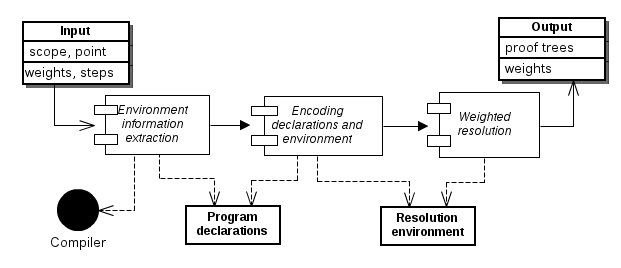
\includegraphics[width=0.45\textwidth]{sav_prez/in_synth_steps}
\caption{InSynth modules}
\label{fig:InSynth_resolution_steps}
\end{figure}

\subsubsection{Environment information extraction}

The first step is the environment information extraction which has the task to extract all usable information about the program.
In the case of Scala programs, the Scala compiler is consulted
\footnote{in the Eclipse IDE integration implementation this is the Scala presentation compiler}
to obtain all local and imported declarations visible at the given program point, which is determined by the typing cursor in the active editor.
The environment extraction automatically assigns weights to all visible declarations according to the distance between the given declaration and the program pointer computed with respect to lines of code and package hierarchy.
The rationale is that the more recent declarations are most likely to be used in the needed expression therefore they should be ranked according to the distance from the given program point.

The number of steps represents a constraint imposed on InSynth in terms of processing time, in order to achieve better responsiveness and ensure a timely termination and suggestions output even in cases of long computations. 

\subsubsection{Encoding the environment}
\label{subsubsec:encoding_the_environment}

The next step of the resolution phase is to encode the environment in the representation which is suitable for the type inhabitation solver to reason about and search for feasible expressions which can be derived from it.

Table \ref{tab:correspondence} shows some examples of how are Scala declarations (and their types) transformed to appropriate representation terms.
The simplified representation of Scala declarations and their types corresponds to the Definition $4.1$ of \textit{ground types} presented in \cite{EPFL-REPORT-170040}.
%PUT HERE def?!
The recursive definition of \textit{ground types} denotes a set of types which include all constants (which correspond to Scala primitive types) and instantiations of constructors (which correspond to Scala generic types) with ground types.
This means that in our resolution process we only consider the instantiated type constructions (e.g. a valid ground type could correspond to Scala types \textit{Int, String, List[String], Map[Int, List[String]]} but not to \textit{Map[X, Y]} where \textit{X, Y} are polymorphic type variables).  

\begin{table}[!ht]
\caption{Correspondence between Scala declarations and proof representation terms}
\centering
{\small
\begin{tabular}{|p{0.22\textwidth}|p{0.20\textwidth}|}
\hline
\textbf{Scala declaration} & \textbf{Proof representation term} \\
\hline
\texttt{val I:Int} & I: $\{\} \rightarrow Int$ \\
\hline
\texttt{def fun(g: Int, f: Int=>Boolean): String} & fun:
$\{ Int, \{ Int \} \rightarrow Boolean \} \rightarrow String$ \\
\hline
\texttt{class A\{ def m(): String \}} & m: $\{A\} \rightarrow String$ \\
\hline
\texttt{class A\{ val s: String \}} & s: $\{A\} \rightarrow String$ \\
\hline
\texttt{def fun(i: Int, c:Char, j: Int): Char} & fun: $(Int, Char) \rightarrow Char$ \\
\hline
% \texttt{def fun(i: Int, c:Char): Char=>Int} & fun: $(Int, Char) \rightarrow Int$ \\
% \hline
\end{tabular}
}
\label{tab:correspondence}
\end{table} 

The environment representation is based on the notion of a type function $f: \{X_1, X_2,\ldots\} \rightarrow Y$ which encodes the information that an expression of type $Y$ can be constructed if a declaration $f$ is used together with expressions of types that belong to the set $X =\{X_1, X_2,\ldots\}$.
More specifically, if expressions $e_i: X_i$ such that $X_i \in X$ where $i=1..|X|$ are available then we can construct an expression $e:Y$ by using those expressions $e_i$ with the declaration $f$ in combination. 

Note that this step produces a representation that sacrifices some information about the language constructs (such as parameter arity, parameter ordering, curring, receiver objects, constructors\ldots) in order to enable more convenient and efficient reasoning with the inhabitation problem solving process (and to make it actually feasible) but also includes corresponding program declarations in order to make the results that use such representation eligible for code reconstruction.

\subsubsection{Weighted resolution}

In order to search for code snippets of the given type, the resolution phase uses theorem proving techniques and reasoning about a similar problem that can be found in type theory, the so-called \textit{type inhabitation problem}, as is defined in Definition \ref{def:inhabitation_problem}.
In the absence of parametric polymorphism, the problem can be seen as the type inhabitation in the simply typed lambda calculus, which is decidable and PSPACE-complete \cite{Urzyczyn:1997:ITL:645893.671612}.

After establishing the connection between program declarations and simplified representation suitable for resolution (or \textit{ground type} terms) in the previous step which encodes the environment (Section \ref{subsubsec:encoding_the_environment}), a calculus for reasoning about the type inhabitation problem is constructed by using only one resolution rule (in  \cite{EPFL-REPORT-170040} it is denoted by \textit{the ground applicative calculus} and it uses multiple rules instead).

\begin{figure}[ht]
\centering{
\inferrule [AppAbs] {\Gamma \vdash f : (\{S_1 \rightarrow T_1\} \cup S_2) \rightarrow T_2 \\ \Gamma \cup \Gamma_{S_1} \vdash h: T_1}
{\Gamma \vdash f(\lambda x_1: ts_1, \ldots \lambda x_n: ts_n. h): S_2 \rightarrow T_2}
\vspace{2mm}
\noindent\begin{minipage}{.26\textwidth}
\begin{equation*}
\Gamma_{S_1} = \{ x_i : ts_i | ts_i \in S_1 \wedge x_i \in \textrm{Fresh} \} 
\end{equation*}
\end{minipage}     
\begin{minipage}{.20\textwidth}  
\begin{equation*}
n = |\Gamma_{S_1}|
\end{equation*}
\end{minipage}
}
\vspace{2mm}
\caption{The calculus rule}
\label{fig:appabs_rule}
\end{figure}

The rule for the calculus construction is depicted in Figure \ref{fig:appabs_rule}.
In combination with the \textit{ground type} representation the \textsc{AppAbs} rule subsumes both the application and abstraction semantics of the lambda calculus (and thus also function composition) in the resolution process.
In order to define starting condition for the resolution process, the \textit{query} \textit{ground type} is added as $q:T \rightarrow \bot$ where $T$ represents the required type of synthesized expressions and $\bot$ represents a fresh type (not usable with the rule for construction of new terms) which is used to denote the end of some expression construction (since $q$, can be instantiated only if an expression of type $T$ itself has been constructed). 

According to the defined calculus the last step of the resolution phase performs the weighted resolution (weights obtained from the information extraction are used to direct the search to more optimal results \cite{EPFL-REPORT-170040}) and produces proof trees which are then used as inputs to the code generation phase. 